% Chapter 3

\chapter{软件开发设计}

\section{概要}
设计要求是:用户输入一张图片后,可以得到相应的标注语句,了解图片语义,生成自然语言解释;在用户输入一句话的时候,可以得到描述这一句话的图片,直观“感受”文字。软件的设计结构如图~\ref{fig:struct}所示。

\begin{figure}[!htbp]
    \centering
    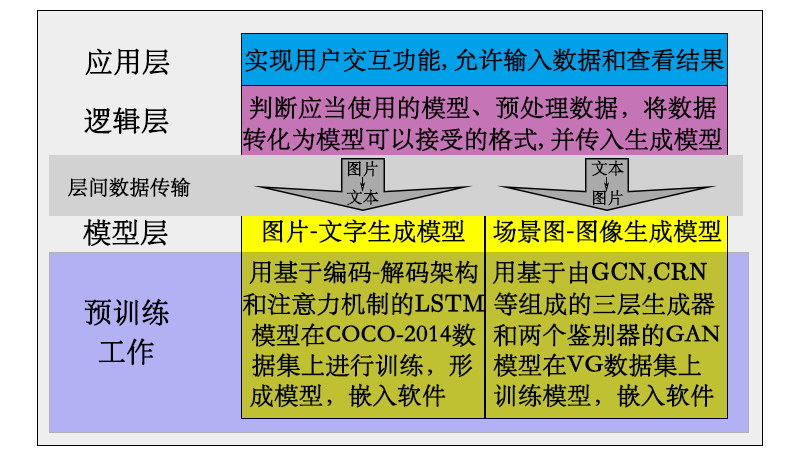
\includegraphics[width=0.9\textwidth]{figures/软件框架.png}
    \caption{软件框架结构}
    \label{fig:struct}
\end{figure}

软件设计主界面使用python的tkinter包来制作。python是一个跨平台语言,用python制作方便产品在不同平台使用。界面中应当可以选择调动两个功能,分别是图片翻译为自然语言和语句翻译为图片。两个功能分别提前训练出成品模型,通过主界面按钮内嵌入的方法,调用对应模型进行计算。

\section{软件模型}
软件分为三个部分,第一部分是软件界面,需要实现简洁明了的操作功能,方便使用。

第二部分是图片标注功能。实现这一功能的模型通过image caption的模型进行训练,算法参照蒙特利尔大学Kevin Xu\upcite{xu2015show}提出的模型进行实现,并经过基于一个或多个数据集进行多个epoch的训练,比较选出表现较好的模型,嵌入到应用中使用。

第三部分是文本生成图片功能。实现这一功能的模型通过一个特殊的GAN模型进行训练,并且要加入后期图片处理算法,以骗过判别器并使其更加真实。这一模型参照卡耐基-梅隆大学Justin Johnson\upcite{Johnson_2018}提出的基于场景双GAN模型配合进行实现,并经过合适的数据集训练,得到表现较好的模型,嵌入到应用当中使用。

为了更好地进行开发与设计,构建了软件的数据流图,方便对软件的结构进行直观的观察。
在软件处理用户操作时,将数据按照数据流图~\ref{fig:dataflow}所示的流程,处理用户提交的文本或者图像,实现翻译功能。

\begin{figure}
    \centering
    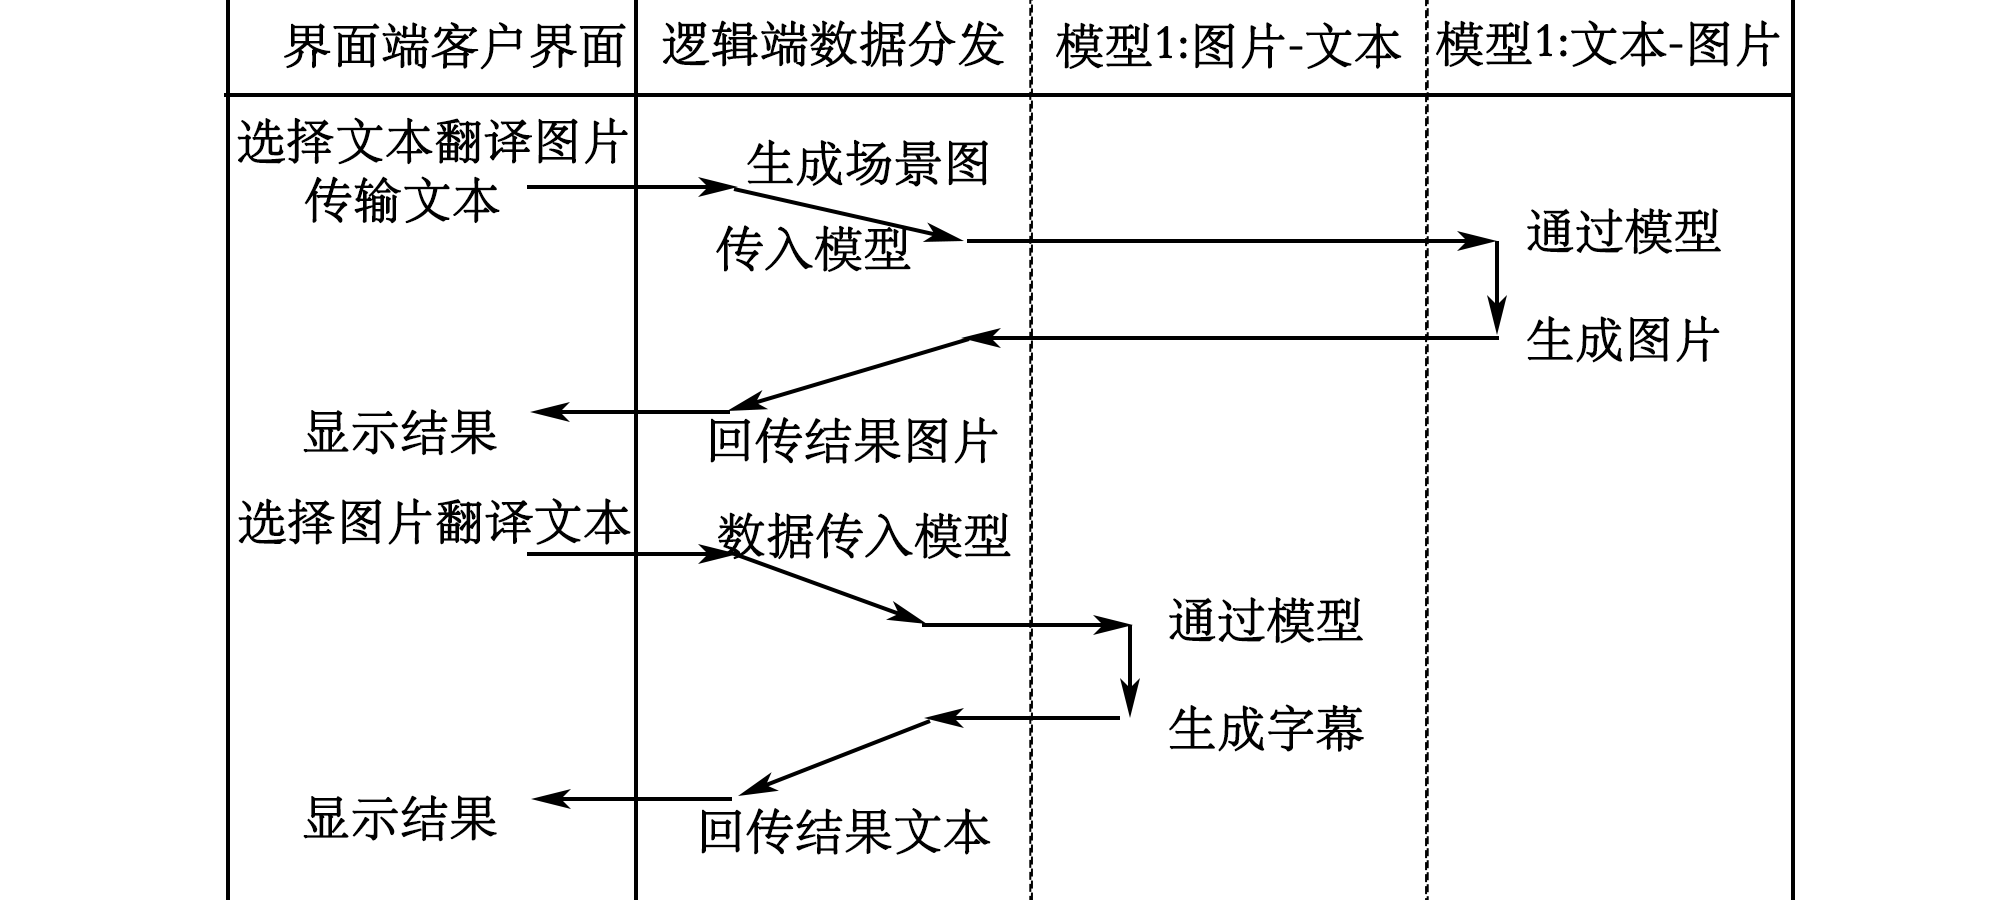
\includegraphics[width=0.9\textwidth]{figures/数据流图.png}
    \caption{本设计的数据流图}
    \label{fig:dataflow}
\end{figure}

\section{变量符号与定义}
文中使用集合如下:
\begin{enumerate}[fullwidth,itemindent=2em,label=\arabic*.]
    \item $O$代表物品(object)的集合;
    \item $C$代表物品目录(catagory)的集合;
    \item $R$代表关系(relationship)的集合;
    \item $E$代表物品-关系-物品组成的边(edge)的集合。
\end{enumerate}

文中脚标定义如下:
\begin{enumerate}[fullwidth,itemindent=2em,label=\arabic*.]
    \item ${}_t$代表LSTM模型中的时序,${}_t$为当前时序,而${}_{t-1}$或${}_{t+1}$为前一或后一时序;
    \item $_f$代表任一函数(使用$f$指代)代入当前操作或模型;
    \item $v_i$在第二个算法中,代表GCN当前层级的节点编号,因为不讨论跨多层关系,所以脚标中不增加时序信息。
\end{enumerate}

文中小写字母对象定义如下:
\begin{enumerate}[fullwidth,itemindent=2em,label=\arabic*.]
    \item $s$指代集合$S$中的元素,其中$S$指代任一集合,如物品集合$O$等,他们通常和集合一起出现;
    \item $c$代表LSTM模型中的细胞(cell),记录细胞当前状态;
    \item $i$代表LSTM模型中的输入门(input),执行LSTM模型中的输入操作;
    \item $o$代表LSTM模型中的输出门(output),执行LSTM模型中的输入操作;
    \item $f$代表LSTM模型中的遗忘门(forget),选择LSTM细胞的部分状态丢失;
    \item $z$代表生成模型中为了骗过判别器、降低生成图片锐度增加的噪声。
\end{enumerate}

文中主要函数定义如下:
\begin{enumerate}[fullwidth,itemindent=2em,label=\arabic*.]
    \item $\phi$代表注意力机制;
    \item $\mathcal{L}$函数代表GAN模型中用作训练目标函数的损失函数;
    \item $f(S,z)$代表自然语言生成图像算法中的目标函数。
\end{enumerate}

\section{软件界面设计}
\subsection{软件例图}
对于预期的软件效果,制作了原型图(图~\ref{fig:UIproto})进行示意。图中,应当出现英文的地方用英文示意,应当出现路径的地方用路径示意,而应当出现中文的地方和说明文字使用中文表述。
\begin{figure}[!htb]
    \centering
    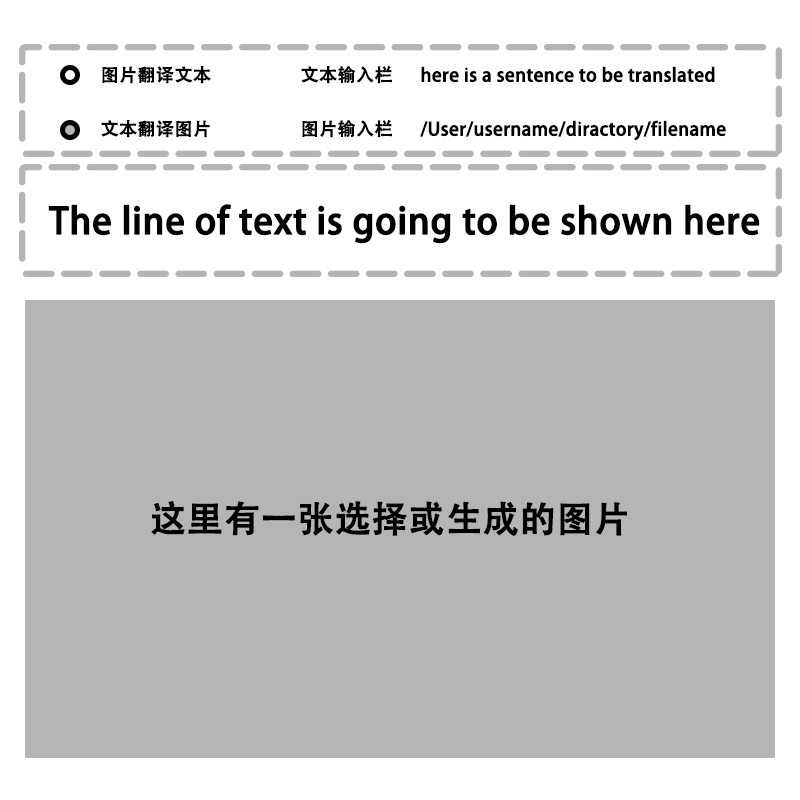
\includegraphics[width=0.8\textwidth]{figures/界面原型图.png}
    \caption{软件界面原型图}
    \label{fig:UIproto}
  \end{figure}

  其中,界面上方由一组两个单选选项的选择栏和两个数据输入栏组成。选项栏的作用是选择当前需要实现的功能,由“图片翻译文本”和“文本翻译图片”两个选项组成;数据输入栏分别是一个文本输入栏和一个文件选择栏,分别对应着文本和图片的输入选择。

  其下是一个明显的按钮,突出的设计可以让用户能轻易明白操作方法,也让用户更有仪式感,能感受到这一操作的划时代意义。

  最下方的大区域是输出区域,根据功能的不同可以输出不同的内容。在选择图像翻译文本功能时,会输出一句话,这一行文字和图片将一起显示,方便对比观察;在选择文本生成图像选项时,将输出生成的图片和原语句,也是为了方便用户观察与分享,表意清晰。

\subsection{软件开发模型}
对开发设计软件的过程,选用了编码-修改模型\upcite{pressman2005software}(Code-fix Model)。如图~\ref{fig:codenfix}所示,在这一模型中不进行计划与建模,先进行编码,调整至用户满意时,发布运行,在出现问题与更新时维护,直到软件生命周期结束为止。

本次软件设计开发的过程是要独立接触一个不熟悉的领域,对于开发者来说不易估计编码需要的时间。深度学习对初学者来说有一个难点:环境安装中很多细节难以把控;并且深度学习的学习过程需要使用多块显卡进行天级时长的训练过程,才可以得到结果。基于上述理由,可以推测算法的实现需要比较长的时间,并且可能一次训练出的算法达不到理想的状态,需要调整模型、重复训练。

\begin{figure}[!htb]
    \centering
    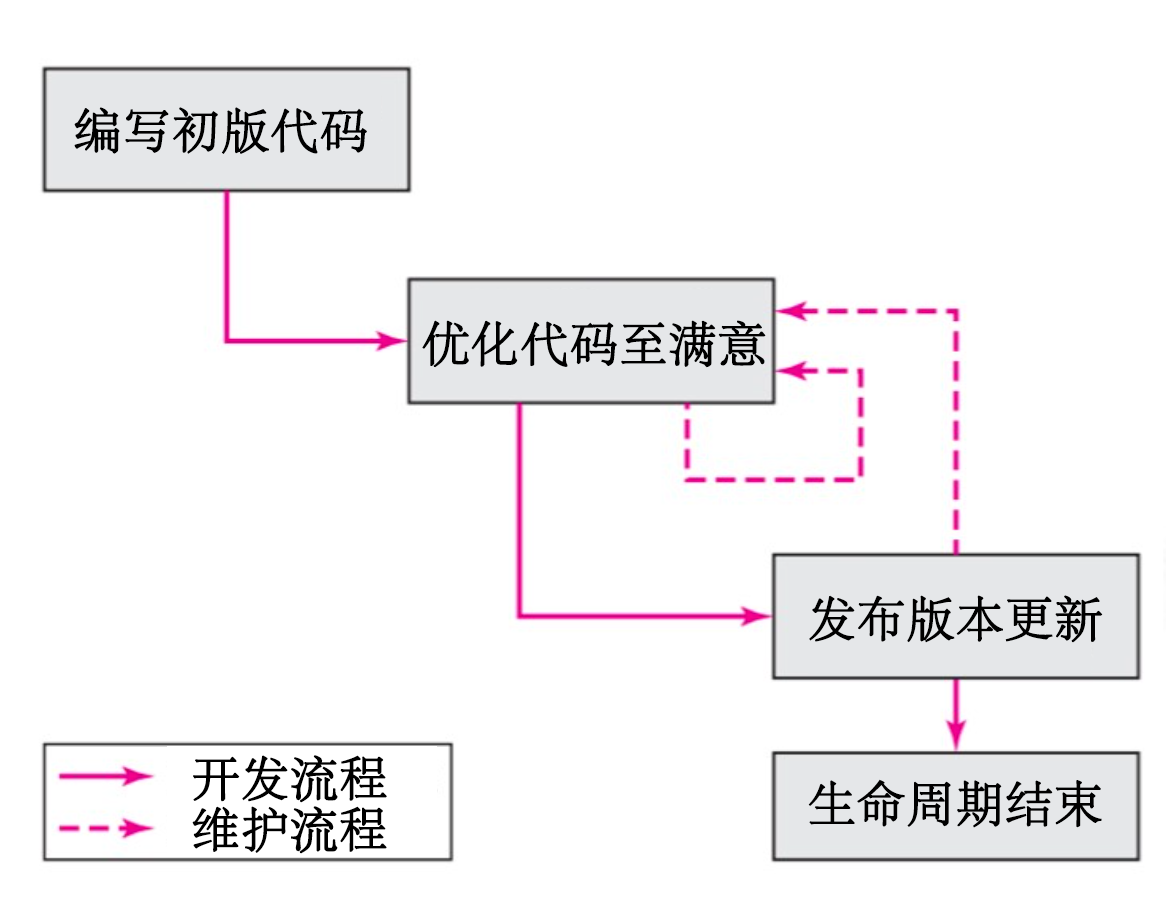
\includegraphics[width=0.6\textwidth]{figures/codeandfix.png}
    \caption{编码-修改模型的基本结构}
    \label{fig:codenfix}
\end{figure}

设计过程中的难点的确是环境安装部分。需要的新虚拟容器因为电脑上旧有的项目擅自修改了环境变量,需要重新安装、整理环境,并且安装合适版本的环境,搭配当前系统,对开源项目进行修改、复现,并在此基础上进行改进。

另外,本软件的模型相对比较简单,是用户界面-调用模型的两层结构,难点在于模型的建立和调整。所以本设计非常适合使用编码-修改模型进行开发。

\section{本章小结}
本章具体地研究了这一设计中所包含的设计细节,并确定了软件构架的结构,为完成代码构建和实验设计打下了基础。

本章内容包含了软件数据流图、用例图,确定了软件开发使用编码-修改模型的开发结构,确定了开发计划的时序,以实验编码-实验运行-客户端编码-实验结果查看-合并模型功能与客户端功能-维护的流程,完成软件的设计与开发。

对于界面的开发,确定了以python语言的tkinter库来编写界面,保证界面清晰易懂。
%{\songti \bfseries 宋体加粗} {\textbf{English}}

%{\songti \itshape 宋体斜体} {\textit{English}}

%%%{\songti \bfseries \itshape 宋体粗斜体} {\textbf{\textit{English}}}

%\section{编译}
%本模板必须使用XeLaTeX + BibTeX编译,否则会直接报错。 本模板支持多个平台,结合sublime/vscode/overleaf都可以使用。